To get a better feeling for the different definitions of a corner, we'll use them for some things that are not directly related to solving LPs.

\subsection*{Convex Hulls}
\begin{Def}(Convex Hull) Let $x_1,\ldots,x_k$ be some vectors in $\R^n$. The convex hull of these vectors in
\[\mbox{CH}(\{x_1,\ldots,x_k\}) = \left\{\sum _{i=1}^k \lambda_i x_i \left| \sum_{i=1}^k \lambda_i =1,\ \lambda_i\geq 0\right.\right\}\]
\end{Def}

Here we generalise the notion of convex combination to use more than two points. Intuitively if we have a bunch of points in 2D we get all the points that lie within the polygon that is spanned by the points on the CH, see figure \ref{Fig:convexHull}.

\begin{figure}[hbt]
\begin{center}
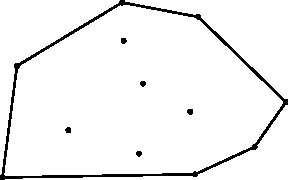
\includegraphics{./images/convex_hull.pdf}
\end{center}
\caption{The convex hull of a set of points}
\label{Fig:convexHull}
\end{figure}

This definition allows us to come up with a different definition of a polyhedron. We already definition \ref{Def:polyhedron}, but the convex hull gives us a more geometric definition.

\begin{Def}[Bounded Polyhedra] A bounded polyhedron lies within a finite bounding box, see figure \ref{Fig:bounded_unbouded}. More formally

\[\forall x\in P,d\in \R^n, \exists \lambda\geq 0: x+\lambda d \not \in P\]

For any line from a point in the polyhedron we eventually leave the polyhedron
\end{Def}

\begin{figure}[hbt]
\begin{center}
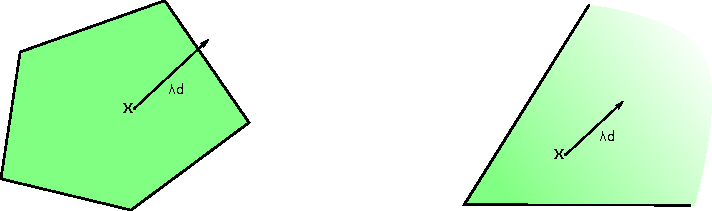
\includegraphics{./images/bounded_unbounded.pdf}
\end{center}
\caption{A bounded (left) and an unbounded (right) polyhedron}
\label{Fig:bounded_unbounded}
\end{figure}

\begin{thm}\label{Thm:CH_polyhedron} Let $P$ be a non-empty bounded polyhedron. Then $P=$CH(extreme points $P$)
\end{thm}

\begin{pr}[Theorem \ref{Thm:CH_polyhedron}]
%\begin{description}
%\item[CH(ex. points of $P$)$\subseteq$ P] 
From the definition we know that all convex combinations of two points are still in P. We generalise to the new kind of convex combination that includes several vectors.

Let $x\in P$. Since $P$ is a polyhedron $x$ is a solution of the system of unequations $Ax\geq b$ (def. \ref{Def:polyhedron}). As before we separate $A$ into the matrix $B$ of active constraint and $D$ of the other constraints, with $Bx=d$, $Dx>f$. If the rank of $B$ is $n$, $x$ is a extreme point by definition and we're done. 

The other possibility is $\rank B=k$ and $k<n$. We use the same trick as in proof \ref{Thm:cornerEquiv} to find two new points. Since the matrix hasn't full rank, there has to be $\delta \neq 0$ such that $B\delta = 0$. As before we build two vectors $x_1 = x+ \epsilon_1 \delta$, $x_2=x-\epsilon_2 \delta$. 

Now we want to get from these points somehow to extreme points, as we want to prove that we can use extreme points to represent every point in $P$. We choose $\epsilon>0$ as the largest value such that $x_1$ is still a feasible solution, that is, we follow a line through $x$ until we reach a boundary of the polyhedron. See figure \ref{Fig:convCombExPoints}

\begin{figure}[hbt]
\begin{center}
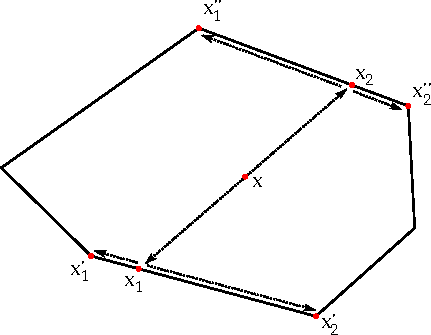
\includegraphics{./images/convex_comb_extr_points.pdf}
\end{center}
\caption{$x$ can be written as a convex combination of $x_1',x_2', x_1''$ and $x_2''$}
\label{Fig:convCombExPoints}
\end{figure}

Such $\epsilon$ has to exist, since the polyhedron is bounded and every line eventually crosses a boundary. Choosing $\epsilon$ like this implies that some constraint $a_i$ in $D$ has to become active for $x_1$ (and $x_2$ by symmetry). Moving in direction $\delta$ doesn't affect the constraints that already were active, since $\delta$ is in the kernel of $B$. So we increase the number of active constraints and can extend $B$. The rank of

\[\begin{pmatrix}B\\ a_i\end{pmatrix}\]

has to be $k+1$ since $\delta$ is orthogonal to all the vectors in $B$. %todo weiter ausführen

Now we can simply do an induction over $k$. Since $x$ is a convex combination of $x_1$ and $x_2$ it has to be in the polyhedron. In particular choose
\begin{align*}
x&=\lambda x_1+(1-\lambda)x_2\\
&=x+\underbrace{\lambda \epsilon_1\delta -(1-\lambda)\epsilon_2\delta}_{\stackrel{!}{=}0}\\
&\Rightarrow \lambda = \frac{\epsilon_2}{\epsilon_1+\epsilon_2}
\end{align*}

Now repeat the process for $x_1$, $x_2$ until you have full rank and are at an extreme point. Since all the points from the beginning can be recursively written by a convex combination of the new points and we end up at an extreme point, the original $x$ can transitively be written by a convex combination of extreme points.
\end{pr}

\begin{cor}\label{Cor:always_extreme_points} Let $P$ be a non-empty bounded polyhedron. Thet the LP $\min cx$ s.t. $x\in P$ has a optimal solution that is an extreme point of $P$.
\end{cor}

\begin{pr} Start with some optimal solution $x^*$. Write is as a convex combination of extreme points 
\[x^* = \sum_{i=1}^x \lambda_i y_i\]
We want to prove that there is a $y_i$ such that

\[cx^* = cy_i\]

Obviously $cy_i\geq 0$. It can't be strictly greater for all $y_i$ or the $\lambda_i$ couldn't all be positive we couldn't find a convex combination for $x_i$. 
\end{pr}

Corollary \ref{Cor:always_extreme_points} gives us the nice result that we can transform the problem of optimising an LP to a discrete problem with finitely many candidate solutions. This will of course be very useful in designing an algorithm for solving them.

\subsection*{Fourier-Motzkin elimination}

In this section we're interested in computing representations of projections of polyhedra. See figure \ref{Fig:polyhedron_proj}

\begin{Def} The projection $x=(\nthings{x})$ onto its first $x$ coordinates is $\pi_k(x) = (x_1,\ldots, x_k)$. 

Let $S\subseteq \R^n$ then the projection on the first $k$ components is

\[\pi_k(S)=\{\pi_k{x}|x\in S\}\]
\end{Def}

Of course that definition is not particularly useful in actually constructing the projection. The Fourier-Motzkin elimination computes the projection for polyhedra. We start with our usual characterisation of a polyhedron $P=\{x|Ax\geq b_i\}$ and want to find a different matrix $A'$ s.t. we get $\pi_{n-1}(P)$. Generalizing to $\pi_k$ is then of course easy.

We want to classify the constraints $a_i$ into three kinds. Let $\overline a = \pi_{n-1}a$ then we can write  

\[P=\left\{x\left| \begin{array}{cr}
\overline a_i\overline x +a_{in}x_n \geq b_i & i\in T_1\\
\overline a_i\overline x +a_{in}x_n \geq b_i & i\in T_2\\
\overline a_i\overline x \geq b_i & i\in T_3\\
\end{array}\right.\right\}\]
\[\forall i\in T_1: a_{in}>0,\ \forall i\in T_2: a_{in}<0,\ \forall i\in T_3: a_{in}=0 \]

Then we can find some scalars such that we can write the polyhedron as

\[P \{i\in T_1 \wedge x_n \geq d_i + f_i \bar x \vee i\in T_2 \wedge x_n \leq d_i + f_i \bar x \vee i\in T_3 \wedge 0 \leq d_i + f_i \bar x\}\]

Then we can write the projection as 

\[Q = \overline P = \{\bar x | d_i+f_i\bar x \leq d_j+f_j\bar x \forall i\in T_2,j\in T_1, \vee d_i+f_i\bar x \geq 0\ \forall i\in T_3\}\]

Herein lies the problem of the algorithm. We introduce a new constraint for every pair of constraints from $T_1,T_2$. Hence in every iteration the number of constraints can grow quadratically.

\begin{pr} To prove that we need to show
\begin{enumerate}
\item $\bar x \in \bar P \Rightarrow x\in Q$. That means 
\[\exists x_n: \left[{\bar x}\atop{x_n}\right] \in P \Rightarrow \max_{i\in T_1} d_i +f_i \bar x \leq x_n \Rightarrow \min_{i\in T_2} d_i+fi\bar x \geq x_n\]
Therefore the first kind of constraints ($i \in T_{1,2}$) are satisfied.
\item $\bar x \in Q \Rightarrow \bar x \in \pi_{n-1}(P)$. Choosing $x_n$ as 
\[x_n \in [\max_{i\in T_1} d_i+f_i \bar x, \min_{i\in T_2} d_i+f_i \bar x]\]
does the trick
\end{enumerate}
\end{pr}

There are a lot of interesting applications for these projections:

\begin{thm} Let $P\in \R^n$ be a polyhedron and $A\in \R^{m\times n}$ be a matrix. Then 
\[\{Ax|x\in P\}\]
is a polyhedron.
\end{thm}

In 2D this is intuitively clear: applying linear transformations on polygons results in distorted, rotated etc. polygons. For higher dimensions it follows from the projections:

\begin{pr} For $P$ we have

\[Q=\{(Ax,x)\in R^{m+n}| x\in P\}\]

is a polyhedron. Then $\pi_m(Q)$ is also a polyhedron.
\end{pr}

\begin{cor} Let $x_1,x_2,\ldots, x_k \in \R^n$, then CH($x_1,x_2,\ldots, x_k$) is a polyhedron\end{cor}

We can use the projections to find the optimal value for an LP (not the optimal solution though). Suppose we're given a LP in the usual form, $\min cx$ s.t. $Ax\geq b$. We construct the following polyhedron

\[P=\{(x_0,\ldots,x_n) | A(x_0,\ldots,x_n)^{\mbox{T}} \geq b \wedge x_0=c(x_0,\ldots,x_n)^{\mbox{T}}\}\]

Define $Q = \pi_1(P)$. We can  find that with the algorithm. If $Q$ is not feasible, $P$ is empty. Else we can choose the biggest $b_i$ such that $x_0\geq b_i$ or the smallest $b_i$ such that $x_0 \leq b_i$, depending on the type of constraints we have. That is the optimal value.

\begin{thm}[Farkas' lemma] Let $A\in \R^{m\times n}$ and $b\in \R^m$. Then either 
\begin{itemize}
\item $\exists x\in R^n: Ax\geq b$ or
\item $\exists y\in R^m, y\geq 0, y^{\mbox{T}}A=0: y\cdot b>0$
\end{itemize}
\end{thm}

This theorem is very nice if we want to check if some system of inequalities is feasible. We just have to find the vector $y$. Thes lemma can be proven by our earlier results. We start with the polygon $P$ and use a projection to get rid of the last dimension of $P$. By that we get another matrix $B$ and another vectior $d$. We get the new inequalities by combining those from the original polyhedron. Instead of actually doing the projection to a lower dimension we can replace the last element by 0. You can show that $[B0]=DA$. You can repeat that proces until you get a matrix $F$ such that $FA=0$. The system is infeasible if you end up with a negative rhs for a constraint, since all lhs will be 0.